\documentclass[aps,preprint,nofootinbib,floatfix]{revtex4-1}
%\documentclass{article}

%\usepackage{nips_2017}

% to compile a camera-ready version, add the [final] option, e.g.:
%\usepackage[final]{nips_2017}

%\usepackage{nicefrac}       % compact symbols for 1/2, etc.
%\usepackage{microtype}      % microtypography
\usepackage{amsmath,amssymb,amsfonts,amsthm,amscd,bm,bbm}
%\usepackage{mathtools}
%\usepackage{printlen}
%\usepackage[inline]{enumitem}
%\usepackage{cite}
%\usepackage{bbm}

\usepackage[pdftex]{graphicx}
\graphicspath{{./figs/}}

\usepackage{algorithmic}
\usepackage{algorithm}
\usepackage[none]{hyphenat}

\hyphenation{op-tical net-works semi-conduc-tor}

\newtheorem{theorem}{Theorem}
\newtheorem{definition}[theorem]{Definition}
\newtheorem{assumption}[theorem]{Assumption}
\newtheorem{lemma}[theorem]{Lemma}
\newtheorem{corollary}[theorem]{Corollary}
\newtheorem{proposition}[theorem]{Proposition}
\newtheorem{conjecture}[theorem]{Conjecture}
\newtheorem{remark}[theorem]{Remark}
\newtheorem{example}{Example}

%% our definitions %%%%%%%%%%%%%%%%%%%%%%%%%%%%%%%%%%%%%%%%%%%%%%%%%%%%%%%%%%%%
\DeclareMathOperator{\aff}{aff}
\DeclareMathOperator{\st}{s.t.}
\DeclareMathOperator{\LC}{LC}
\DeclareMathOperator{\affnot}{aff_0}
\DeclareMathOperator{\conv}{conv}
\DeclareMathOperator{\relint}{relint}
\DeclareMathOperator{\vol}{vol}
\DeclareMathOperator{\range}{range}
\DeclareMathOperator{\image}{im}
\DeclareMathOperator{\nullspace}{null}
\DeclareMathOperator{\area}{area}
\DeclareMathOperator{\vspan}{span}
\DeclareMathOperator{\id}{Id}
\DeclareMathOperator{\cond}{cond}
\DeclareMathOperator{\prox}{prox}
\DeclareMathOperator*{\argmax}{arg\,max}
\DeclareMathOperator*{\argmin}{arg\,min}
\DeclareMathOperator*{\minimize}{minimize}
\DeclareMathOperator{\diag}{diag}
\DeclareMathOperator{\Tr}{Tr}

\newcommand\Energy{\mathcal{E}}
\newcommand\E{\mathbb{E}}
\newcommand\kk{K}
\newcommand\kkk{h}
\newcommand\Hk{{\mathcal{H}}_{\kk}}
\newcommand\HH{\mathcal{H}}
\newcommand\C{{\mathcal{C}}}
\newcommand\OO{{\mathcal{O}}}
%\newcommand\Zt{\widetilde{Z}}
\newcommand\Zt{Y}
%\newcommand{\Ind}[1]{\delta_{#1}}
\newcommand{\Ind}[1]{\mathbbm{1}_{#1}}


\begin{document}


\title{Nonparametric Clustering from  Energy Statistics}

\author{Guilherme Fran\c ca}
\email{guifranca@gmail.com} 
%\affiliation{Johns Hopkins University}

\author{Joshua T. Vogelstein}
\email{jovo@jhu.edu}

\affiliation{Johns Hopkins University}


\begin{abstract}
Energy statistics provides a nonparametric test for equality of distributions.
It was proposed by 
Sz\' ekely in the 80's
inspired by the Newtonian gravitational potential from classical mechanics. 
Energy statistics
was further generalized to probability 
distributions on arbitrary metric spaces,
and more recently a connection with reproducing kernel Hilbert spaces 
was established.
Nevertheless, although extensively used by the statistics community, it
has not been previously incorporated in machine learning problems.
In this paper, we consider the problem of clustering data from
an energy statistics theory perspective.
We provide a precise mathematical formulation yielding
a quadratically constrained quadratic program (QCQP).
We show the equivalence between the energy statistics clustering
formulation 
and the kernel $k$-means optimization problem (not to be confused with
kernel $k$-means algorithm). 
Therefore, our results imply a first principles derivation of 
kernel $k$-means problem
from energy statistics theory, thus bringing this important 
clustering method into a formal statistical framework.
Moreover, energy statistics is nonparametric, it usually fixes
the kernel choice,
and if prior information is available
it can be easily incorporated in the kernel construction.
We propose an iterative algorithm
to find local optimizers of the aforementioned QCQP based on the 
energy change
of moving points to different clusters. This algorithm 
is different but has the same computational cost as kernel $k$-means 
algorithm.
We compare it to
kernel $k$-means, standard $k$-means, and GMM/EM algorithms by 
providing carefully designed numerical experiments. The results
show that, in general, this algorithm outperforms
these most used clustering algorithms.
\end{abstract}

\maketitle


\section{Introduction}

Energy statistics is based on the energy distance between probability
distributions, which provides a notion of statistical potential energy
to statistical observations, in close analogy to Newton's gravitational
potential in classical mechanics. 
It provides a nonparametric test for equality of distribution,
such that minimum energy is achieved under equality of 
distributions. 
We refer the reader 
to \cite{Szkely2013}, and references therein, for an overview.
Energy statistics has been applied to several goodness-of-fit 
hypothesis tests, 
multi-sample tests of equality of distributions, analysis of variance
\cite{RizzoVariance}, and (nonlinear)
dependence tests through
distance covariance and distance correlation, which generalizes the Pearson
correlation coefficient. 
Moreover, energy statistics  was applied
to hierarchical clustering \cite{RizzoClustering} by extending Ward's
method of minimum variance.

More recently, distance covariance was 
generalized from Euclidean
spaces to metric spaces of strong negative type \cite{Lyons}.
Furthermore, a unifying framework establishing an equivalence
between generalized energy distances to maximum
mean discrepancies (MMD), which are distances between embeddings of
distributions in reproducing kernel Hilbert spaces (RKHS), was
established \cite{Sejdinovic2013}. This important work provides the missing
link
between techniques commonly used in the statistics literature, regarding
energy statistics, and techniques
commonly used in machine learning.

Given a dataset $\mathbb{X} = \{x_1,\dotsc,x_n \}$, where each
data point $x_i$ lives in a space $\mathcal{X}$, the clustering
problem consists in grouping these points into $k$ groups $\{
\C_1,\C_2,\dotsc,\C_k \}$, such that
points belonging to the same group are more ``similar'' to each other
than to points in  other groups. This intuitive notion already assumes
a ``metric'' able to measure the similarity between points. Clustering
is an unsupervised method, and one of the most important problems in machine
learning since it provides the first step towards automatically constructing
labels for previously unseen data. In practice
$k$-means is arguably the most used algorithm, and gaussian 
mixture models (GMM) through the expectation
maximization (EM) algorithm is also often used. Both are parametric, making 
strong assumptions about
the distribution of the data (isotropy and normality), and it assumes
that data points
lie in Euclidean space, $\mathcal{X} = \mathbb{R}^D$, hence
the similarity is based on Euclidean metric, 
$\| x_i - x_j \|^2 = (x_i - x_j)^\top(x_i-x_j) = 
\sum_{\ell=1}^D (x_{i,\ell} - x_{j,\ell})^2$. These algorithms provide
a good quality clustering when data is linearly separable in Euclidean space,
i.e. there is a clear resolution in the cluster centers
and points from different clusters do not overlap considerably.

To account for nonlinearly separable data, which may live
in an arbitrary non-Euclidean space, kernel methods are usually employed.
If a so-called Mercer kernel $\kk: \mathcal{X}\times \mathcal{X} \to \mathbb{R}$
is available, which is a symmetric and positive definite 
function, it guarantees that there exists a map $\varphi : \mathcal{X} \to
\mathcal{H}$ where $\mathcal{H}$ is a Hilbert space \cite{Mercer}. 
One can thus
compute similarities between data point through the inner product of
the feature space $\mathcal{H}$ and 
perform clustering in $\mathcal{H}$. The convenience of a Mercer
kernel is that the map $\varphi$ is only used implicitly, i.e. one
does not need to know $\varphi$, since the inner
of product of $\mathcal{H}$ can be computed only 
based on the kernel function $\kk(\cdot, \cdot)$ which acts on the original
space $\mathcal{X}$. 
This technique is known as the kernel trick.  
Kernel $k$-means problem 
is exactly $k$-means in the feature space
\cite{Smola,Girolami} (see also \cite{Filippone} for a survey of clustering
methods).
To cluster data that is not linearly
separable in $\mathcal{X}$,
kernel based methods exploit the nonlinear structure provided by
the kernel function, which implicitly maps data points to a usually higher
dimensional feature 
space, with the hope that they becomes separable by 
forming well-defined groups.
The choice of
kernel is crucial, and yet there is no principled method
for this. One must rely on ad hoc methods to find an appropriate kernel
which is data dependent.
As it stands, kernel $k$-means problem is an heuristic approach to clustering
in the sense that it is not derived from a statistical theory. 

The main contribution of this paper is to provide a consistent formulation
to clustering based on energy statistics theory. 
The original goal is to provide a nonparametric
clustering method, since energy distance is nonparametric.
The basis of our work is the theory developed in 
\cite{Sejdinovic2013} which establishes an equivalence between energy
distance and RKHS. 
Based on this and on the multi-sample test
for equality of distributions, we show that
there is only one possible clustering optimization
problem consistent with the energy statistics formulation. 
We then show that this 
optimization problem is equivalent to a quadratically constrained quadratic
program (QCQP), which has the same trace maximization
form as kernel $k$-means,
spectral clustering, and some well-known graph partitioning problems
\cite{Dhillon2,Dhillon}. We show the equivalence between this approach
and kernel $k$-means optimization problem, implying that
the later can actually be derived from energy statistics, thus
bringing this important clustering method into a unified statistical theory.
However, it is important to note that 
energy statistics fixes a kernel to begin with.
From an algorithmic perspective, our contribution is to 
provide an iterative algorithm, which is different but has the same
complexity as kernel $k$-means algorithm. Our numerical results
provide compelling evidence that this algorithm 
is more accurate and robust than kernel $k$-means algorithm.
Moreover, these experiments 
puts in evidence the nonparametric aspect of energy
statistics based clustering, since it is able to perform accurately
on data having very different distributions, contrary to $k$-means and
GMM for instance.

Our work is organized as follows. In section~\ref{sec:background} we review
the necessary background on energy statistics and RKHS.
Section~\ref{sec:clustering_theory} contains the main theoretical 
results of this paper,
where we consider a clustering theory based on energy statistics, leading
to a QCQP which is NP-hard.
In section~\ref{sec:twoclass} we consider a simple example in one dimension,
where we propose an algorithm which requires no initialization.
In section~\ref{sec:algo} we briefly review kernel $k$-means algorithm,
and propose a new iterative algorithm to solve this QCQP.
Section~\ref{sec:numerics} contains some carefully designed numerical
experiments indicating that this algorithm outperforms kernel
$k$-means, standard $k$-means, and GMM/EM algorithms.
Our final conclusions are presented in section~\ref{sec:conclusion}.



%%%%%%%%%%%%%%%%%%%%%%%%%%%%%%%%%%%%%%%%%%%%%%%%%%%%%%%%%%%%%%%%%%%%%%%%%%%%%%%
\section{Background on Energy Statistics and RKHS}
\label{sec:background}

In this section we briefly review the main concepts from energy
statistics and its relation to reproducing kernel Hilbert spaces 
(RKHS) which form the basis of our work.
For more details we refer the reader
to \cite{Szkely2013} and \cite{Sejdinovic2013}.

Consider random variables in $\mathbb{R}^D$ 
such that $X,X' \stackrel{iid}{\sim} P$ and 
$Y,Y' \stackrel{iid}{\sim} Q$, where $P$ and $Q$ are cumulative
distribution functions with finite first moments. 
The quantity \cite{Szkely2013}
\begin{equation}
\label{eq:energy}
\Energy(P, Q) \equiv 2 \E \| X - Y\| - \E \| X - X' \| - \E \| Y - Y' \|,
\end{equation}
called \emph{energy distance}, 
is rotational invariant and nonnegative, $\Energy(P,Q) \ge 0$, where
equality
to zero holds if and only if $P = Q$.
Above, $\| \cdot \|$ denotes the
Euclidean norm in $\mathbb{R}^D$. 
Energy distance
provides a characterization of equality of distributions, and
$\Energy^{1/2}$ is
a metric on the space of distributions.

The energy distance can be generalized as, for instance,
\begin{equation}
\label{eq:energy2}
\Energy_\alpha(P, Q) \equiv 
2 \E \| X - Y\|^{\alpha} - \E \| X - X' \|^{\alpha} - 
\E \| Y - Y' \|^{\alpha},
\end{equation}
where $0<\alpha\le 2$. This quantity is also nonnegative,
$\Energy_\alpha(P,Q) \ge 0$. Furthermore, for $0<\alpha<2$ we have that
$\Energy_\alpha(P,Q) = 0$ if and only if $P=Q$, while for $\alpha=2$ 
we have $\Energy_2(P,Q) = 2\| \E(X) - \E(Y) \|^2$, showing that
equality to zero only requires
equality of the means, and thus $\Energy_2(P,Q)=0$ does 
not imply equality of distributions.

It is important to 
mention that \eqref{eq:energy2} can be even further generalized.
Let $X, Y \in \mathcal{X}$,  where $\mathcal{X}$ is an arbitrary space endowed
with a \emph{semimetric of negative type}
$\rho: \mathcal{X}\times\mathcal{X} \to \mathbb{R}$, which is required
to satisfy
\begin{equation}
\label{eq:negative_type}
\sum_{i,j=1}^n c_i c_j \rho(X_i, X_j) \le 0,
\end{equation}
where $X_i \in \mathcal{X}$, and $c_i \in \mathbb{R}$ such that
$\sum_{i=1}^n c_i = 0$. Then, $\mathcal{X}$ is called a \emph{space of
negative type}.
We can thus replace $\mathbb{R}^D \to \mathcal{X}$ and 
$\| X - Y \| \to \rho(X , Y)$ in the definition \eqref{eq:energy}, obtaining
the generalized energy distance
\begin{equation}
\label{eq:energy3}
\Energy(P, Q) \equiv 2 \E \rho(X,Y) - \E \rho(X, X') - \E \rho(Y,Y').
\end{equation}
For spaces of negative type, there exists a Hilbert space $\mathcal{H}$ and
a map $\varphi: \mathcal{X} \to
\mathcal{H}$ such that
$\rho(X, Y) = \| \varphi(X) - \varphi(Y) \|_{\mathcal{H}}^2$, which
allows us to compute quantities related to probability distributions over
$\mathcal{X}$ in the Hilbert space $\mathcal{H}$.
Even though the semimetric 
$\rho$ may not satisfy the triangle inequality, 
$\rho^{1/2}$ does since it can be shown to be a legit metric. 

There is an equivalence between energy distance, 
commonly used in statistics,
and distances between embeddings of distributions in 
RKHS, commonly used in machine learning. 
This equivalence was established
in \cite{Sejdinovic2013}. Let us first recall the definition of
RKHS. Let $\HH$ be a Hilbert space of real-valued functions
over $\mathcal{X}$. A function 
$\kk : \mathcal{X} \times \mathcal{X} \to 
\mathbb{R}$ is a reproducing kernel of $\HH$ if it satisfies
the following two conditions:
\begin{enumerate}
\item $\kkk_x \equiv \kk(\cdot, x) \in \HH$ 
for all $x \in \mathcal{X}$.
\item $\langle \kkk_x, f \rangle_{\HH} = f(x)$ for
all $x\in\mathcal{X}$ and $f\in \HH$.
\end{enumerate}
In other words, for any $x \in \mathcal{X}$ and any function $f \in \HH$,
there is a unique 
$\kkk_x \in \HH$ that reproduces $f(x)$ through the inner product
of $\HH$.
If such a \emph{kernel} 
function $\kk$ exists, then $\HH$ is called a RKHS. The above two 
properties immediately imply that $\kk$ is symmetric and positive
definite. Indeed, notice that
$\langle \kkk_x, \kkk_y \rangle = \kkk_y(x) = \kk(x,y)$, and since
this inner product is real,
$\langle \kkk_x, \kkk_y \rangle^* = \langle \kkk_y, \kkk_x \rangle = 
\langle \kkk_x, \kkk_y \rangle$, we immediately have that
the kernel is symmetric,
$\kk(y,x) = \kk(y,x)$. Moreover, for any $w \in
\HH$ we can write $w = \sum_{i=1}^n c_i \kkk_{x_i}$, where
$\{ \kkk_{x_i} \}_{i=1}^n$ is a basis of $\HH$. It follows that
$\langle w, w \rangle_{\HH}  = \sum_{i,j=1}^n c_i c_j \kk(x_i,x_j) \ge 0$,
showing that the kernel is positive definite. If $G$ is a matrix with
elements $G_{ij} = \kk(x_i,x_j)$, this is equivalent to $G$ being
positive semidefinite; $v^\top G \, v \ge 0$ for any vector
$v \in \mathbb{R}^n$.

The Moore-Aronszajn theorem 
\cite{Aronszajn}
establishes the converse of the above paragraph. 
For every symmetric
and positive definite function $\kk: \mathcal{X}\times \mathcal{X} \to
\mathbb{R}$, there is an associated RKHS $\Hk$ 
with reproducing
kernel $\kk$. The map $\varphi: x \mapsto \kkk_x \in \Hk$ is called
the canonical \emph{feature map}. Given a kernel $\kk$,
this theorem enables us to define an embedding of a probability measure
$P$ into the RKHS as follows: $P \mapsto \kkk_P \in
\Hk$ such that 
$\int f(x) d P(x) = \langle f, \kkk_P \rangle$ for all $f \in \Hk$,
or alternatively, $\kkk_P \equiv \int \kk( \, \cdot \,, x)  d P(x)$. 
We can now  introduce the 
notion of distance between two probability measures using the inner product
of $\Hk$. This is called the maximum mean discrepancy (MMD) and
is given by
\begin{equation}\label{eq:mmd}
\gamma_\kk(P,Q) \equiv \| \kkk_P - \kkk_Q \|_{\Hk},
\end{equation}
which can also be written as \cite{Gretton2012}
\begin{equation}\label{eq:mmd2}
\gamma_\kk^2(P,Q) = \E \kk(X,X') + \E \kk(Y,Y') - 2 \E \kk(X, Y)
\end{equation}
where $X,X' \stackrel{iid}{\sim} P$ and $Y,Y'\stackrel{iid}{\sim} Q$.
From the equality between \eqref{eq:mmd} and \eqref{eq:mmd2} we also
have 
\begin{equation}\label{eq:inner_data}
\langle \kkk_P, \kkk_Q \rangle_{\Hk} = \E \, \kk(X, Y).
\end{equation}
Thus, in practice, we can estimate the inner product between  
embedded distributions 
by averaging the kernel function over sampled data.

The following important result shows that semimetrics of negative
type and symmetric positive semidefinite kernels are closely related
\cite{Berg1984}. Let $\rho: \mathcal{X} \times \mathcal{X} \to \mathbb{R}$,
and $x_0 \in \mathcal{X}$ an arbitrary but fixed point.
Define
\begin{equation}
\label{eq:kernel_semimetric}
\kk(x,y) \equiv 
\tfrac{1}{2} \left[  \rho(x,x_0) + \rho(y,x_0) - \rho(x,y)\right].
\end{equation}
Then, it can be shown that 
$\kk$ is positive definite if and only if $\rho$ is a semimetric
of negative type
\eqref{eq:negative_type}.
Here we have a family of kernels, one for each choice of $x_0$. Conversely,
if $\rho$ is a semimetric of negative type and $\kk$ is a kernel in this
family, then 
\begin{equation}
\label{eq:gen_kernel}
\begin{split}
\rho(x,y) &= \kk(x,x) + \kk(y,y) -2\kk(x,y) \\
&=  \| \kkk_x - \kkk_y \|^2_{\Hk},
\end{split}
\end{equation}
and the canonical feature map 
$\varphi: x \mapsto \kkk_x$ is injective \cite{Sejdinovic2013}.
When these conditions are satisfied, we say that the kernel $\kk$ 
generates the semimetric $\rho$. 
If two different kernels generate the same $\rho$ they are
equivalent kernels.

Now we can state the equivalence between energy distance $\Energy$ and
inner products on RKHS, which is one of the main results of
\cite{Sejdinovic2013}. If $\rho$ is a semimetric
of negative type and $\kk$ a kernel that generates $\rho$, then
replacing \eqref{eq:gen_kernel} into
\eqref{eq:energy3}, and using \eqref{eq:mmd2}, yields
\begin{equation} \label{eq:Erho}
\Energy(P, Q) = 
2 \left[ \E \, \kk(X, X') + \E \, \kk(Y, Y') - 2\E \, \kk(X, Y)\right] 
= 2 \gamma_\kk^2(P,Q) .
\end{equation}
Since $\gamma_k^2(P, Q) = \| \kkk_P - \kkk_Q \|^2_{\Hk}$ we
can compute the energy distance using the inner product of $\Hk$. Moreover,
this can be computed from the data according to \eqref{eq:inner_data}.

Finally, let us recall the main formulas for test statistic
of equality of distributions \cite{Szkely2013}. 
Assume we have data $\mathbb{X} = \{ x_1,\dotsc, x_n \}$, where
$x_i \in \mathcal{X}$, and $\mathcal{X}$ is a space of negative type.
Consider a partition $\mathbb{X} = \bigcup_{j=1}^k \C_j$, with
$\C_i \cap \C_j = \emptyset$.
Each expectation in 
\eqref{eq:energy3}
can be computed 
through the function
\begin{equation}
\label{eq:g_def}
g (\C_i, \C_j) \equiv 
\dfrac{1}{n_i n_j}
\sum_{x \in \C_i} 
\sum_{y \in \C_j} \rho(x, y)
\end{equation}
where $n_i = |\C_i|$ is the number of elements in 
$\C_i$. 
The \emph{within energy dispersion} is defined by
\begin{equation}
\label{eq:within}
W \equiv
\sum_{j=1}^{k} \dfrac{n_j}{2} g(\C_j, \C_j),
\end{equation}
and the \emph{between-sample energy statistic} is defined by
\begin{equation}
\label{eq:between}
S \equiv
\sum_{1 \le  i < j \le k } \dfrac{n_i n_{j}}{2 n} \left[
2 g(\C_i, \C_j) - 
g(\C_i, \C_i) - 
g(\C_j, \C_j)
\right],
\end{equation}
where $n = \sum_{j=1}^k n_j$.
Given a set of distributions
$\{ P_j\}_{j=1}^k$, where $x \in \C_j$ if and only if $x \sim P_j$, 
the quantity $S$ provides
a \emph{nonparametric test statistic} for equality of distributions
\cite{Szkely2013}.
When the sample size is large enough, $n\to \infty$,
under the null hypothesis $H_0: P_1=P_2=\dotsm=P_k$ we have that
$S\to 0$, 
and under
the alternative hypothesis $H_1: P_i \ne P_j$ for at least two $i\ne j$, 
we have that $S \to \infty$.
This test is nonparametric in the sense that it does not make any assumptions
about the distributions $P_j$.

One can make the analogy 
that every data point $ x \in \C_j$ form a massive body, 
whose total mass is characterized by the distribution function $P_j$.
The quantity $S$ is thus a potential
energy of the from $S(P_1,\dotsc,P_k)$ which measures how different
these
mass distributions are, and achieves the ground state
$S=0$ when all bodies have the same mass distribution. The potential energy
$S$ increases as bodies have different mass distributions.



%%%%%%%%%%%%%%%%%%%%%%%%%%%%%%%%%%%%%%%%%%%%%%%%%%%%%%%%%%%%%%%%%%%%%%%%%%%%%%%
\section{Clustering Based on Energy Statistics}
\label{sec:clustering_theory}

This section contains the main theoretical results of this paper, where 
we formulate an optimization problem for clustering 
based on energy statistics and RKHS introduced in the previous section.

Due to the test statistic \eqref{eq:between} for equality of distributions,
the obvious
criterion for clustering data is to 
maximize $S$, which makes 
each cluster as different
as possible from the other ones.
In other words, given a set of points coming from different probability
distributions, $S$ should attain a maximum when each point is correctly
classified as belonging to the cluster associated to its probability
distribution.
The following 
straightforward result
shows that maximizing \eqref{eq:between} is, however, equivalent to minimizing
\eqref{eq:within} which has a more convenient form.

\begin{proposition}
\label{th:minimize}
Let $\mathbb{X} = \{x_1,\dotsc,x_n\}$ where each data point
$x_i$ lives in a space $\mathcal{X}$ endowed with a semimetric $\rho:
\mathcal{X}\times\mathcal{X} \to \mathbb{R}$ of
negative type \eqref{eq:negative_type}. For a fixed integer $k$,
the partition
$\mathbb{X} = \bigcup_{j=1}^k \C_j$, where $\C_i \cap C_j = \emptyset$ for
all $i\ne j$, maximizes \eqref{eq:between} if and only if
\begin{equation}
\label{eq:minimize}
\min_{\C_1,\dotsc,C_k  } W(
\C_1, \dotsc, \C_k),
\end{equation}
where $W$ is given by \eqref{eq:within}.
\end{proposition}
\begin{proof}
From \eqref{eq:within} and \eqref{eq:between}
we have
\begin{equation}
\begin{split}
S + W &= 
\dfrac{1}{2n} \sum_{\substack{i,j=1 \\ i\ne j}}^k n_i n_j g(\C_i, \C_j)
+ \dfrac{1}{2n} \sum_{i=1}^{k} 
\bigg[ n - 
\sum_{j\ne i = 1}^k n_j \bigg] 
n_i g(\C_i, \C_i) 
\\
& = \dfrac{1}{2n} \sum_{i,j=1}^k n_i n_j g(\C_i, \C_j)
= \dfrac{1}{2n} \sum_{x \in \mathbb{X}} \sum_{y \in \mathbb{X}} \rho(x,y)
= \dfrac{n}{2} g(\mathbb{X}, \mathbb{X}).
\end{split}
\end{equation}
Note that the right hand side of this equation 
only depends on the pooled data, so it is a constant
independent of the choice of partition. Therefore, maximizing
$S$ over the choice of partition is equivalent to minimizing~$W$.
\end{proof}

Therefore, for a given $k$, the clustering problem amounts to
finding the best partition of the data by solving~\eqref{eq:minimize}.
Notice that this is a hard assignment clustering problem as partitions
are disjoint.

Now we show how to formulate problem \eqref{eq:minimize} in the corresponding
RKHS.
Based on 
\eqref{eq:kernel_semimetric} and \eqref{eq:gen_kernel}, assume that 
the kernel $\kk: \mathcal{X} \times \mathcal{X} \to \mathbb{R}$ 
generates $\rho$. 
Let us define  the Gram matrix
\begin{equation}
\label{eq:kernel_matrix}
G \equiv \begin{pmatrix}
\kk(x_1,x_1) & \kk(x_1,x_2) & \dotsm & \kk(x_1,x_n) \\
\kk(x_2,x_1) & \kk(x_2,x_2) & \dotsm & \kk(x_2,x_n) \\
\vdots & \vdots & \ddots  & \vdots \\
\kk(x_n,x_1) & \kk(x_n,x_2) & \dotsm & \kk(x_n,x_n) 
\end{pmatrix} .
\end{equation}
Let $Z \in \{ 0,1 \}^{n\times k}$ be the label matrix, 
with only one nonvanishing entry per row, 
indicating to which cluster (column)
each point (row) belongs to. This matrix satisfy
$Z^\top Z = D$ where the diagonal matrix 
$D = \diag( n_1,\dotsc, n_k )$  contains
the number of points in each cluster. Let us also introduce the rescaled
matrix  $Y \equiv Z D^{-1/2}$. In component form they are given by
\begin{equation}
\label{eq:label_matrix}
Z_{ij} \equiv \begin{cases}
1 & \mbox{if $x_i \in \C_j$ } \\
0 & \mbox{otherwise}
\end{cases} \qquad
\Zt_{ij} \equiv \begin{cases}
\tfrac{1}{\sqrt{n_j}} & \mbox{if $x_i \in \C_j$ } \\
0 & \mbox{otherwise}
\end{cases} .
\end{equation}
Throughout the paper, we use the notation $M_{i\bullet}$ to denote
the $i$th row of a matrix $M$, and $M_{\bullet j}$ denotes its $j$th column.
Our next result reveals the optimization problem behind \eqref{eq:minimize},
which is NP-hard since
it is a quadratically constrained quadratic program (QCQP).

\begin{proposition} 
\label{th:qcqp2}
The problem \eqref{eq:minimize} is equivalent to
\begin{equation}
\label{eq:qcqp2}
\max_{\Zt} \Tr \left( \Zt^\top G \, \Zt \right)  \qquad
\mbox{s.t. $\Zt \ge 0$, $\Zt^\top \Zt = I$, 
$\Zt \Zt^\top \bm{e} = \bm{e}$},
\end{equation}
where $\bm{e} = (1,1,\dots,1)^\top \in \mathbb{R}^n$ is the all-ones vector,
and $G$ is the Gram matrix \eqref{eq:kernel_matrix}.
\end{proposition}
\begin{proof}
From 
\eqref{eq:gen_kernel},
\eqref{eq:g_def}, and
\eqref{eq:within}
we have
\begin{equation}
\label{eq:W2}
W(\C_1,\dotsc,\C_k  )
= \dfrac{1}{2} \sum_{j=1}^k \dfrac{1}{n_j} \sum_{x,y \in \C_j} \rho(x,y)
= \sum_{j=1}^k \sum_{x \in \C_j}  \bigg(
\kk(x,x) - \dfrac{1}{n_j} \sum_{y \in \C_j} \kk(x,y) \bigg).
\end{equation}
Note that the first term does not contribute to the optimization problem,
since it is a global term that does not depend which partition is chosen. 
Therefore, minimizing \eqref{eq:W2} is equivalent to
\begin{equation}
\label{eq:max_prob}
\max_{ \C_1,\dotsc,\C_k } 
\sum_{j=1}^k \dfrac{1}{n_j} \sum_{x,y\in C_j} \kk(x,y) .
\end{equation}
But 
\begin{equation}
\sum_{x, y \in \C_j} \kk(x, y) =
\sum_{p=1}^{n} \sum_{q=1}^{n} Z_{pj} Z_{qj} G_{pq} = 
(Z^\top G \, Z)_{jj},
\end{equation}
where we used the definitions \eqref{eq:kernel_matrix} and
\eqref{eq:label_matrix}. Thus, the objective function in 
\eqref{eq:max_prob} is equal to
$\Tr \left( D^{-1} Z^\top G Z \right)$. Now we can
use the cyclic property
of the trace, and by the own definition of the matrix $Z$
in \eqref{eq:label_matrix}, we obtain the following integer
programing problem:
\begin{equation}\label{eq:qcqp}
\max_{Z} \Tr\Big( \big( Z D^{-1/2}\big)^\top G 
\big( ZD^{-1/2} \big) 
\Big) \quad
\mbox{s.t. $Z_{ij} \in \{0,1\}$, $\sum_{j=1}^k Z_{ij} = 1$, 
$\sum_{i=1}^n Z_{ij} = n_j$.}
\end{equation}

Now we write this in terms of the matrix $Y = Z D^{-1/2}$.
The objective function immediately becomes
$\Tr\left( Y^\top G \, Y\right)$. Notice that the above constraints
imply that $Z^T Z = D$, where $D=\diag(n_1,\dotsc,n_k)$, which in turn gives
$D^{-1/2} Y^T Y D^{-1/2} = D$, or $Y^\top Y = I$. 
Also, every entry of $Y$ is positive by definition,
$Y \ge 0$. Now it only remains to show the last 
constraint in \eqref{eq:qcqp2}, which comes from the last
constraint in \eqref{eq:qcqp}. In matrix form this reads
$Z^T \bm{e} = D \bm{e}$. Replacing $Z=YD^{1/2}$ we have
$Y^\top \bm{e} = D^{1/2} \bm{e}$. Multiplying this last equation
on the left by $Y$, and noticing
that $Y D^{1/2} \bm{e} = Z \bm{e} = \bm{e}$, we finally obtain
$Y Y^\top \bm{e} = \bm{e}$. Therefore, the optimization 
problem \eqref{eq:qcqp} is equivalent
to \eqref{eq:qcqp2} .
\end{proof}

Based on Proposition~\ref{th:qcqp2}, to group data $\{ x_1,\dotsc,x_n \}$
into  $k$ clusters, we first compute the Gram matrix
$G$ and then 
solve the optimization problem \eqref{eq:qcqp2} for $\Zt \in
\mathbb{R}^{n\times k}$. The $i$th row
of $\Zt$ will contain a single nonzero element in some $j$th column,
indicating that $x_i \in \C_j$. 
Problem \eqref{eq:qcqp2} is NP-hard and there
are few methods
available to solve it directly,
which is computational prohibitive even for small datasets.
However, one can find approximate solutions by relaxing some 
of the constraints, or obtaining a relaxed SDP version of it.
For instance, the relaxed problem
\begin{equation}
\max_{Y} \Tr \left( Y^\top G \, Y \right) \quad \mbox{s.t. $Y^\top Y = I$}
\end{equation}
has a well-known closed form solution $Y^\star = U R$, where the
columns of $U$ contain the leading $k$ eigenvectors of $G$ corresponding
to the $k$ largest eigenvalues $\lambda_1\ge \lambda_2\ge\dotsc\ge\lambda_k$, 
and
$R \in \mathbb{R}^{k\times k}$ is an arbitrary orthogonal matrix. 
The resulting
optimal objective function is given by
$\max \Tr \left( {Y^\star}^\top G \, Y^\star \right)  = 
\sum_{i=1}^k \lambda_i$. One might then normalize and threshold the rows
of $Y^\star$, or even better, following \cite{NgJordan} we can normalize the
rows of $Y^\star$ and apply standard $k$-means on this matrix where each
row is considered as a data point.
This is the same 
procedure done in spectral clustering on the (normalized) Laplacian
of the graph defined by a similarity matrix.
However, computing eigenvectors of a very large matrix
can be problematic, and usually iterative methods are preferred.
We will propose an iterative method to find approximate solutions
to \eqref{eq:qcqp2} in section~\ref{sec:algo}.

It is important to note 
that the previous theory for clustering based on energy statistics
is valid for data living in an \emph{arbitrary} space of negative type.
This clustering method is
\emph{nonparametric} since it does not make any assumptions
about 
the distribution of the data, nor the metric space where data belongs
to,
contrary to $k$-means and gaussian mixture models (GMM), for example.
Moreover, this approach \emph{does not} require the concept of the 
\emph{cluster mean},
which can be ill-defined for some types of data, such as images for
instance. Since no mean is involved, the method should also be 
robust to outliers.
%This method is quite general and makes very few
%assumptions about the data. 
If one uses the traditional energy distance
defined in \eqref{eq:energy}, 
then $\rho(x,y) = \| x - y\|$, and this fixes the kernel
through \eqref{eq:kernel_semimetric}. In the same way, 
for data living in more general
metric spaces $(\mathcal{X}, \rho)$, the corresponding semimetric $\rho$ fixes
the kernel.
In practice, however,
the clustering quality strongly depend on the choice of a suitable
$\rho$ which is what measures the similarity between different data points,
and is equivalent to choosing an appropriate kernel.
Nevertheless, if prior knowledge is available for choosing $\rho$, 
this can easily be taken into account.

One may wonder how energy statistics clustering 
relates to the well-known kernel $k$-means problem\footnote{
When we refer to kernel $k$-means problem we mean specifically 
the optimization
problem \eqref{eq:kernel_kmeans}, which should not be confused with
kernel $k$-means algorithm, which is just one possible recipe to solve
\eqref{eq:kernel_kmeans}.}.
We now address this question.
For a positive semidefinite $G$, there exists a map
$\varphi: \mathcal{X} \to \HH_\kk$ such that
$\kk(x,y) = \varphi(x)^\top \varphi(y)$. The kernel $k$-means optimization
problem,
in feature space,
is defined by
\begin{equation}
\label{eq:kernel_kmeans}
\min_{\C_1,\dotsc,\C_k}\bigg\{ 
J(\C_1,\dots,\C_k) \equiv  \sum_{j=1}^k
\sum_{x \in \C_j} \| \varphi(x) - \varphi(\mu_j) \|^2
\bigg\},
\end{equation}
where $\mu_j = \tfrac{1}{n_j} \sum_{x \in \C_j} x$ is the  mean of cluster
$\C_j$ in the ambient space. Notice that the above objective function
is strongly tied to the idea of minimizing distances between points
and cluster centers, which arises from $k$-means objective function.
It is known \cite{Dhillon2,Dhillon} that problem \eqref{eq:kernel_kmeans} 
is equivalent to a QCQP in the same form as
\eqref{eq:qcqp2}. The next result makes this explicit, showing that
\eqref{eq:minimize} and \eqref{eq:kernel_kmeans} are actually equivalent.

\begin{proposition}
\label{th:kernel_kmeans}
The clustering optimization problem
\eqref{eq:minimize} based on energy statistics 
is equivalent to the kernel $k$-means optimization problem
\eqref{eq:kernel_kmeans}, and both are equivalent to \eqref{eq:qcqp2}.
\end{proposition}
\begin{proof}
Notice that $\| \varphi(x) - \varphi(\mu_j) \|^2 = \varphi(x)^\top \varphi(x)
- 2 \varphi(x)^\top \varphi(\mu_j) + \varphi(\mu_j)^\top \varphi(\mu_j)$,
therefore
\begin{equation}
\label{eq:J}
J = \sum_{j=1}^k \sum_{x\in\C_j} \bigg(
\kk(x,x) - 
\dfrac{2}{n_j} \sum_{y\in \C_j} \kk(x,y) + \dfrac{1}{n_j^2}
\sum_{y,z \in \C_j} \kk(y,z) \bigg).
\end{equation}
The first term is global so it does not contribute to the optimization
problem. Notice that the third term gives
$\sum_{x\in\C_j} \tfrac{1}{n_j^2} \sum_{y,z\in\C_j} \kk(y,z) =
\tfrac{1}{n_j}\sum_{y,z\in\C_j} \kk(y,z)$, which is the same as
the second term. Thus, the kernel $k$-means optimization problem
\eqref{eq:kernel_kmeans} is equivalent to
\begin{equation}
\min_{\C_1,\dotsc,\C_k} \bigg\{ J(\C_1,\dotsc,\C_k) = \max_{\C_1,\dotsc,\C_k}
\sum_{j=1}^k \dfrac{1}{n_j} \sum_{x,y \in\C_j} \kk(x,y) \bigg\}
\end{equation}
which is exactly the same as 
\eqref{eq:max_prob} from the energy statistics formulation. Therefore,
once the kernel $\kk$ is fixed, the function 
$W$ given by \eqref{eq:within} is the same
as $J$ in \eqref{eq:kernel_kmeans}.
The remaining of the proof proceeds as 
already shown in the proof of Proposition~\ref{th:qcqp2}, leading to
the optimization problem in the form \eqref{eq:qcqp2}.
\end{proof}

The above result shows that 
kernel $k$-means problem is actually a consequence
of energy statistics. In this vein, kernel $k$-means is part of a
statistical framework where we are maximizing distances between probability
distributions.

As shown in \cite{Dhillon}, kernel $k$-means, spectral clustering,
and graph partitioning problems such as ratio association, ratio cut, and
normalized cut are all equivalent to a QCQP of the form \eqref{eq:qcqp2}, thus
one can use kernel $k$-means algorithm to solve these problems as well.
This correspondence involves a weighted version of \eqref{eq:qcqp2}, that
for the sake of completeness demonstrate next.


%%%%%%%%%%%%%%%%%%%%%%%%%%%%%%%%%%%%%%%%%%%%%%%%%%%%%%%%%%%%%%%%%%%%%%%%%%%%%%%
\subsection{Clustering Based on Weighted Energy Statistics}

Now we generalize the formulas from energy statistics to incorporate
weights associated to each data point.
Let $w(x)$ be a weight function for the point $x \in \mathbb{X}$.
We can generalize \eqref{eq:g_def} as follows:
\begin{equation}
\label{eq:g_def2}
g(\C_i, \C_j) \equiv \dfrac{1}{s_i s_j} \sum_{x\in \C_i}\sum_{y\in\C_j}
w(x)w(y) \rho(x,y), \qquad s_i \equiv \sum_{x\in\C_i} w(x).
\end{equation}
Now we replace this function in the formulas \eqref{eq:within} and
\eqref{eq:between}, with 
$n_i \to s_i$ and $n \to s$ where $s = \sum_{j=1}^k s_j$,
to obtain a weighted version of energy test statistic. With these
changes, Proposition~\ref{th:minimize} remains the unnaltered, so the
clustering problem becomes
\begin{equation}
\label{eq:minimize2}
\min_{\C_1, \dotsc, \C_k} 
\bigg\{
W(\C_1,\dotsc,\C_k) \equiv \sum_{j=1}^k \dfrac{s_j}{2} g(\C_j,\C_j)
\bigg\}
\end{equation}
where now $g$ is given by \eqref{eq:g_def2}. 
Let us define the following matrices and vector:
\begin{equation}
\label{eq:weighted_matrices}
Y_{ij} \equiv \begin{cases}
\tfrac{1}{\sqrt{s_j}} & \mbox{if $x_i \in \C_j$} \\
0 & \mbox{otherwise}
\end{cases}, \qquad
\mathcal{W} \equiv \diag(w_1,\dotsc,w_n), \qquad
H \equiv \mathcal{W}^{1/2} Y, \qquad
\bm{\omega} \equiv \mathcal{W} \bm{e},
\end{equation}
where $w_i = w(x_i)$ and $\bm{e} \in \mathbb{R}^n$ is the all-ones
vector. Now we can show the analogous of
Proposition~\ref{th:qcqp2} to the case of \eqref{eq:minimize2}.

\begin{proposition}
\label{th:qcqp3}
The weighted version of energy statistics clustering given by
problem \eqref{eq:minimize2} is equivalent to
\begin{equation}
\label{eq:qcqp3}
\max_H \Tr \left\{ H^\top (\mathcal{W}^{1/2} G \mathcal{W}^{1/2}) H  \right\}
\qquad \mbox{s.t. $H \ge 0$, $H^\top H = I$, $H H^\top \bm{\omega} =
\bm{\omega}$,}
\end{equation}
where $G$ is the Gram matrix \eqref{eq:kernel_matrix} and the other quantities
are defined in 
\eqref{eq:weighted_matrices}.
\end{proposition}
\begin{proof}
Replacing \eqref{eq:gen_kernel} and elimating the global terms which 
do not contribute, the optimization problem \eqref{eq:minimize2}
becomes 
\begin{equation}
\max_{\C_1,\dotsc,\C_k} \sum_{j=1}^k \dfrac{1}{s_j}
\sum_{x\in\C_j}\sum_{y\in\C_j} w(x)w(y) \kk(x,y) . 
\end{equation}
This 
objective function can be written as
\begin{equation}
\begin{split}
\sum_{j=1}^k \dfrac{1}{s_j} 
\sum_{p=1}^n \sum_{q=1}^n 
w_p w_q Z_{pj} Z_{qj} G_{pq} &= 
\sum_{j=1}^k 
\sum_{p=1}^n \sum_{q=1}^n 
\dfrac{Z^\top_{jp}\sqrt{w_p}}{\sqrt{s_j}} w_p^{1/2} G_{pq} w_q^{1/2} 
\dfrac{\sqrt{w_q} Z_{qj}}{\sqrt{s_j}} \\
&= 
\sum_{j=1}^k \left(H^\top \mathcal{W}^{1/2} G \mathcal{W}^{1/2} H\right)_{jj}
\\
&= \Tr\left( H^\top \mathcal{W}^{1/2} G \mathcal{W}^{1/2} H  \right).
\end{split}
\end{equation}
To obtain the constraints, note that $H_{ij} \ge 0$ by definition, and
\begin{equation}
(H^\top H)_{ij} = \sum_{\ell=1}^n 
Y_{\ell i} \mathcal{W}_{\ell \ell} Y_{\ell j } = 
\dfrac{1}{\sqrt{s_i}\sqrt{s_j}} \sum_{\ell=1}^n w_\ell Z_{\ell i} Z_{\ell j}
= \dfrac{\delta_{ij}}{s_i} \sum_{\ell=1}^n w_\ell Z_{\ell i} = \delta_{ij},
\end{equation}
therefore $H^\top H = I$. This is a constraint on the rows of $H$.
Now we obtain a condition on the columns
of $H$. Observe that
\begin{equation}
\left(H^\top H\right)_{pq} = \sqrt{w_p w_q}\sum_{j=1}^k \dfrac{Z_{pj}
Z_{qj}}{s_j} = \begin{cases}
\dfrac{\sqrt{w_p w_q}}{s_i} & \mbox{if both $x_p,x_q \in \C_i$} \\
0 & \mbox{otherwise}.
\end{cases}
\end{equation}
Therefore, $(H^\top H \mathcal{W}^{1/2})_{pq} = \sqrt{w_p} \, w_q s_i^{-1}$
if both points $x_p$ and $x_q$ belong to the same cluster, which
we denote by $\C_i$ for some $i=1,\dotsc,k$, and 
$(H^\top H \mathcal{W}^{1/2})_{pq} = 0 $ otherwise. Thus, the $p$th
line of this matrix is nonzero only on entries corresponding to points
that are in the same cluster as $x_p$. If we sum over the columns of this
line we obtain $\sqrt{w_p} s_i^{-1} \sum_{q=1}^n w_q Z_{qi} = \sqrt{w_p}$,
or equivalently $H H^\top \mathcal{W}^{1/2} \bm{e} = \mathcal{W}^{1/2} \bm{e}$,
which gives the constraint $H H^\top \bm{\omega} = \bm{\omega}$.
\end{proof}


%%%%%%%%%%%%%%%%%%%%%%%%%%%%%%%%%%%%%%%%%%%%%%%%%%%%%%%%%%%%%%%%%%%%%%%%%%%%%%%
\subsection{Connection with Graph Partioning}

The relation between kernel $k$-means and graph partitioning problems
was already established \cite{Dhillon}. We repeat a similar analysis
due to the relation of these problems to
energy statistics and RKHS, which may provide a different perspective.

Consider a graph $\mathcal{G} = (\mathcal{V}, \mathcal{E}, \mathcal{A})$,
where $\mathcal{V}$ is the set of vertices, $\mathcal{E}$ the set of edges,
and $\mathcal{A}$ is an affinity matrix of the graph 
that measure the 
similarities between pairs of nodes. Thus, $\mathcal{A}_{ij} \ne 0$
if $(i,j) \in \mathcal{E}$, and $\mathcal{A}_{ij} = 0$ otherwise.
We also associate weights to every vertex, 
$w_i = w(i)$ for $i \in \mathcal{V}$, and let $s_j = \sum_{ i \in \C_j} w_i$,
where $\C_j \subseteq \mathcal{V}$ is one partition of $\mathcal{V}$.
Let
\begin{equation}
\textnormal{links}(\C_\ell, \C_m) \equiv 
\sum_{i\in \C_\ell, j\in \C_m } A_{ij} .
\end{equation}
We want to partition the set of vertices $\mathcal{V}$ into $k$ disjoint
subsets, $\mathcal{V} = \bigcup_{j=1}^k \C_j $. 
The generalized ratio association problem is given by
\begin{equation}
\label{eq:assoc}
\max_{\C_i,\dots,\C_k} \sum_{j=1}^k \dfrac{\textnormal{links}(\C_j,\C_j)}{s_j},
\end{equation}
and maximizes the within cluster association.
The generalized ratio cut problem
\begin{equation}
\label{eq:cut}
\min_{\C_i,\dots,\C_k} \sum_{j=1}^k
\dfrac{\textnormal{links}(\C_j,\mathcal{V} \backslash \C_j)}{s_j},
\end{equation}
minimizes the cut between clusters. These two problems are equivalent,
in analogous way as minimizing \eqref{eq:within} is equivalent to
maximizing \eqref{eq:between}, as shown in Proposition~\ref{th:minimize}.
Here this is due to the equality
$\textnormal{links}(\C_j,\mathcal{V} \backslash \C_j)=
\textnormal{links}(\C_j,\mathcal{V}) - \textnormal{links}(\C_j,\C_j)$.
Several graph partitioning methods 
\cite{Kernighan,Malik,Chan,Yu}
can be seen as a particular
case of \eqref{eq:assoc} or \eqref{eq:cut}.

Consider \eqref{eq:assoc}, whose objective function can be written as
\begin{equation}
\sum_{j=1}^k \dfrac{1}{s_j} \sum_{p \in \C_j} \sum_{q \in \C_j}
\mathcal{A}_{pq} = \sum_{j=1}^k \sum_{p=1}^n \sum_{q=1}^n 
\dfrac{Z^\top_{jp}}{\sqrt{s_j}} \mathcal{A}_{pq} \dfrac{Z_{qj}}{\sqrt{s_j}}
= \Tr\left( Y^\top \mathcal{A} Y \right)
\end{equation}
with $Z$ defined in \eqref{eq:label_matrix} and $Y$ in
\eqref{eq:weighted_matrices}. To make the analogy with \eqref{eq:qcqp3}
explicit,  problem \eqref{eq:assoc} is equivalent to
\begin{equation}
\max_H \Tr\left( H^\top \mathcal{W}^{-1/2} \mathcal{A} \mathcal{W}^{-1/2} H 
\right) \qquad \mbox{s.t. $H\ge 0$, $H^\top H = I$, $H H^\top
\bm{\omega}=\bm{\omega}$}.
\end{equation}
Therefore, this is exactly the same problem as weighted energy statistics
clustering \eqref{eq:qcqp3}, with 
$G = \mathcal{W}^{-1} \mathcal{A} \mathcal{W}^{-1}$. Assuming this
matrix is positive semidefinite, this generates a semimetric
\eqref{eq:gen_kernel} for graphs given by
\begin{equation}
\label{eq:metric_graphs}
\rho(i,j) = 
\dfrac{\mathcal{A}_{ii}}{w_i^{2}}
+\dfrac{\mathcal{A}_{jj}}{w_j^{2}}
-\dfrac{2 \mathcal{A}_{ij}}{w_i w_j} \qquad\mbox{or}\qquad
\rho(i,j) = -\dfrac{2 \mathcal{A}_{ij}}{w_i w_j}
\end{equation}
for vertices $i,j \in \mathcal{V}$, and 
where in the second equation we assume the graph has no self-loops,
$\mathcal{A}_{ii} = 0$. Using \eqref{eq:metric_graphs} 
in \eqref{eq:g_def}--\eqref{eq:between}
allows one to use energy statistics theory for inference
over populations of graphs.


%%%%%%%%%%%%%%%%%%%%%%%%%%%%%%%%%%%%%%%%%%%%%%%%%%%%%%%%%%%%%%%%%%%%%%%%%%%%%%%
\section{Two-Class Problem in One Dimension}
\label{sec:twoclass}

Before stating a general algorithm to solve \eqref{eq:qcqp2}, 
let us first consider the simplest possible case which
is one-dimensional data and a two-class problem. This will be usefull to test
energy statistics clustering on a simple setting.

Fixing
$\rho(x,y) = |x - y|$ according to \eqref{eq:energy}, we can actually compute 
\eqref{eq:g_def} in $\OO(n \log n)$ and find
a direct solution to \eqref{eq:minimize}. 
This is done by noticing that
\begin{equation}
\begin{aligned}
|x - y|  &= (x-y)\Ind{x \ge y} -
(x-y) \Ind{x < y}  \\
&= 
x \left( \Ind{x \ge y} - \Ind{x < y} \right)  + 
y \left( \Ind{y > x} - \Ind{y \le x} \right)  ,
\end{aligned}
\end{equation}
where we have the indicator function defined as
$\Ind{A}=1$ if $A$ is true, and $\Ind{A}=0$ otherwise. 
Let $\C$ be a partition with
$n$ elements. Using the above distance in \eqref{eq:g_def} we have
\begin{equation}
\label{eq:g_ind}
g\left(\C,\C\right) = \dfrac{1}{n^2} \sum_{x \in \C} 
\sum_{y \in \C} 
x \left(
\Ind{x \ge y} + \Ind{y > x} - 
\Ind{x \ge y}-\Ind{x < y} \right) .
\end{equation}
The sum over $y$ can be eliminated since each term in
the parenthesis is simply counting the number of elements in $\C$ that satisfy
the condition of the indicator function. Assuming
that we first order the data inside the partition, obtaining
$\bar{\C} = [ x_j \in \C: x_1 \le x_2 \le \dotsm \le x_{n}]$, we
can write \eqref{eq:g_ind} in the following simple form:
\begin{equation}
\label{eq:g1d}
g\left(\bar{\C}, \bar{\C}\right) = 
\dfrac{2}{n^2} \sum_{\ell=1}^n (2\ell - 1 - n) x_\ell .
\end{equation}
Note that the cost of computing 
\eqref{eq:g1d}
is $\OO(n)$, and the cost of
sorting the data
is at the most $\OO(n\log n)$.
Assuming that each partition is ordered  $\mathbb{X} = \bigcup_{j=1}^k
\bar{\C}_j$, but notice that the entire data set $\mathbb{X}$ does not 
need to be necessarily ordered, the within energy dispersion
\eqref{eq:within} can be written as
\begin{equation}
\label{eq:w1d}
W\left( \bar{\C}_1,\dotsc,\bar{\C}_k \right) = 
\sum_{j=1}^k \sum_{\ell=1}^{n_j} \dfrac{2\ell - 1 - n_j}{n_j} \, x_\ell.
\end{equation}

For a two-class problem, we can use \eqref{eq:w1d} to cluster data
through a simple algorithm 
as follows. We first order
the entire dataset $\mathbb{X} \to \bar{\mathbb{X}}$. Then 
we compute \eqref{eq:w1d} for each possible split of $\bar{\mathbb{X}}$
and pick the point which gives the minimum value of $W$. 
This procedure is described in Algorithm~\ref{algo1d}. 
Notice that
this method does not require any initialization,
however,
it only works for one-dimensional data with Euclidean distance. The total
complexity of the algorithm is $\OO(n\log n + n^2) = \OO(n^2)$.

\begin{figure}
\begin{algorithm}[H]\vspace{.5em}
\begin{algorithmic}[1]
\INPUT data $\mathbb{X}$
\OUTPUT label matrix $Z$
\STATE sort $\mathbb{X}$ obtaining 
$\bar{\mathbb{X}}= [ x_1,\dotsc,x_n ]$
    \FOR{$j\in [ 1,\dotsc,n ]$}
        \STATE Let $\bar{\C}_1^{(j)} = [x_i: i=1,\dotsc,j]$ and 
                $\bar{\C}_2^{(j)} = [x_i : i=j+1,\dotsc,n]$
        \STATE  
            $W^{(j)} \leftarrow W \big( \bar{\C}_1^{(j)},\bar{\C}_2^{(j)}  
            \big)$ from \eqref{eq:w1d}
    \ENDFOR
    \STATE $j^\star \leftarrow \argmin_j W^{(j)}$ 
    \STATE $Z_{j\bullet} \leftarrow (1,0) $ if $j\le j^\star$, and
           $Z_{j\bullet} \leftarrow (0,1)$ otherwise, for $j=1,\dotsc,n$
\end{algorithmic}
\caption{
\label{algo1d}
Approximate solution to \eqref{eq:minimize} 
for a two-class problem in one dimension. \hspace{\fill}
}
\end{algorithm}
\end{figure}

Assuming the true label matrix $Z$ is available, a direct
measure of how different the estimated matrix $\hat{Z}$ 
is from $Z$, up to label
permutations, is given by
\begin{equation}
\label{eq:accuracy}
\textnormal{accuracy}(\hat{Z}) = \max_\sigma 
\dfrac{1}{n}\sum_{i=1}^n\sum_{j=1}^k \hat{Z}_{i \sigma(j)} Z_{ij}
\end{equation}
where $\sigma$ is a permutation
of the $k$ cluster groups. 
The accuracy is always between $[0,1]$, where
$1$ corresponds to all points correctly clustered, and 
$0$ to all points wrongly clustered.
For a two-class problem with equal
number of points in each cluster, the value $1/2$ correspond
to chance.

\begin{figure}
\begin{minipage}{0.49\textwidth}
\hspace{1cm}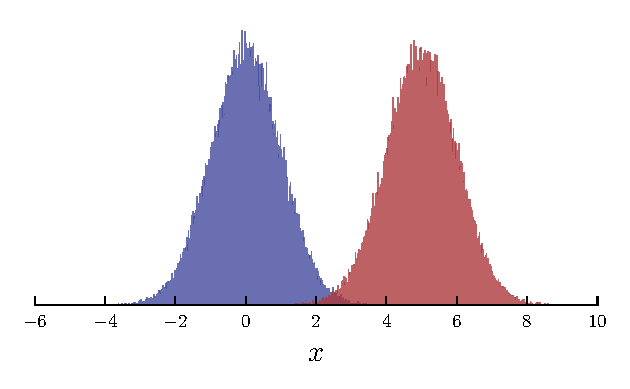
\includegraphics[width=.6\textwidth]{hist_normal.pdf}\\[-.5em]
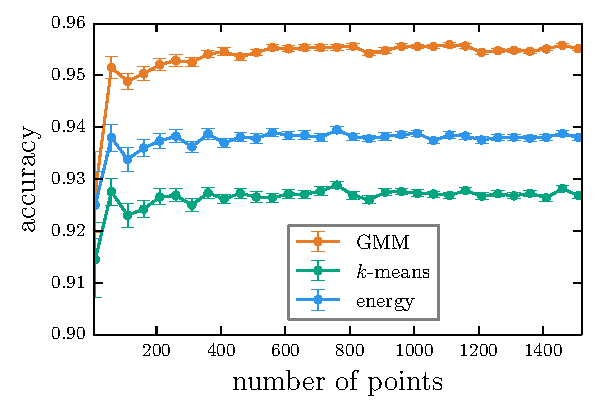
\includegraphics[width=\textwidth]{gauss1d.pdf}\\[-1em]
(a)
\end{minipage}
\begin{minipage}{0.49\textwidth}
\hspace{1cm}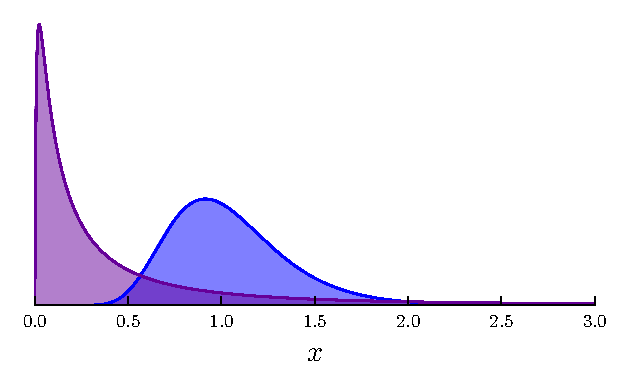
\includegraphics[width=.6\textwidth]{hist_lognormal.pdf}\\[-.5em]
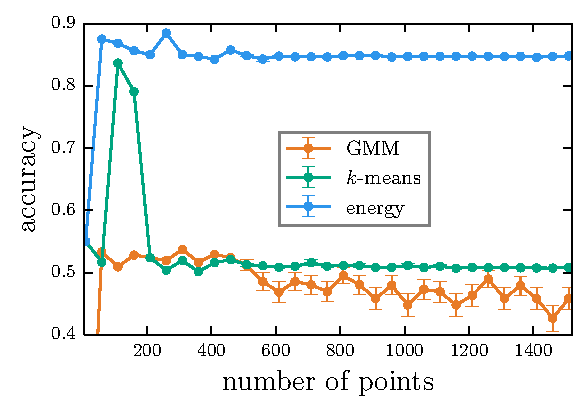
\includegraphics[width=\textwidth]{loggauss1d.pdf}\\[-1em]
(b)
\end{minipage}
\caption{
\label{fig:1d}
Energy statistics clustering by Algorithm~\ref{algo1d},
compared to $k$-means and GMM.
Both clusters
have the same number of points ($x$-axis), 
which are increased in each experiment.
We sample $100$ times from the distributions in the histograms and
the $y$-axis is the average value of the clustering 
accuracy \eqref{eq:accuracy} (errorbars are standard error).
(a) 
$x\sim \tfrac{1}{2}\left[ \mathcal{N}(\mu_1,\sigma_1) +
\mathcal{N}(\mu_2,\sigma_2)  \right]$,  
$\mu_1 = 0$,
$\mu_2 = 5$,
$\sigma_1 = 1$, and
$\sigma_2 = 2$.
(b) 
$x\sim \tfrac{1}{2}\left[ e^{\mathcal{N}(\mu_1,\sigma_1)} +
e^{\mathcal{N}(\mu_2,\sigma_2)}  \right]$,  
$\mu_1 = 0$,
$\mu_2 = -1.5$,
$\sigma_1 = 0.3$, and
$\sigma_2 = 1.5$. 
}
\end{figure}

Let us consider two simple experiments with equal number of points
in each cluster. 
We keep increasing the number of points in the clusters for each experiment, 
and cluster the data using Algorithm~\ref{algo1d}. 
We also cluster the same data set
with GMM, through EM algorithm, and with standard $k$-means. In both of these
cases we use the initialization from $k$-means++ \cite{Vassilvitskii} 
and we run the algorithms
few times with different initializations and choose the answer
with best objective function value. We use \eqref{eq:accuracy} to measure
the clustering quality. Furthermore, we pick $100$ different samples
for each configuration, and show the average accuracy with errorbars indicating
the standard error.
In  Fig.~\ref{fig:1d}a 
we have data from normal distributions,
where we can see that all the three methods
perform closely, with a slight advantage of GMM, as expected, since
it is the true model for the data. Energy statistics performs slightly better
than $k$-means in this experiment. Now in Fig~\ref{fig:1d}b
we consider one example of 
data from lognormal distributions. We can see that energy
statistics clustering through Algorithm~\ref{algo1d} provides a huge 
improvement
compared to both GMM and $k$-means, which basically cluster at chance
in this case.
GMM is worst than chance since sometimes it 
is not able to estimate the parameters, thus giving zero
accuracy.
These two simple experiments illustrate
how energy statistics based clustering is nonparametric, being able
to provide high quality clustering in settings where data comes
from very different distributions.




%%%%%%%%%%%%%%%%%%%%%%%%%%%%%%%%%%%%%%%%%%%%%%%%%%%%%%%%%%%%%%%%%%%%%%%%%%%%%%%
\section{Iterative Algorithm for Energy Statistics Clustering}
\label{sec:algo}

In this section we will introduce a new iterative algorithm to find a local
maximizer of the QCQP \eqref{eq:qcqp2}, however, due to 
Proposition~\ref{th:kernel_kmeans} we can also find an approximate
solution by the well-known kernel $k$-means algorithm, which 
for convenience
will also be restated in the present context.
First, let us introduce some base notation.

Consider the optimization problem 
written in the form \eqref{eq:max_prob} as follows:
\begin{equation}
\label{eq:maxQ}
\max_{\{ \C_1,\dotsc,\C_k \}} 
\bigg\{ Q = \sum_{j=1}^k \dfrac{Q_j}{n_j}  \bigg\},
\qquad Q_j = \sum_{x,y\in\C_j} \kk(x,y),
\end{equation}
where $Q_j$ represents an internal energy cost of cluster $\C_j$, and
$Q$ is the total energy cost where each individual cluster cost 
is weighted by the inverse
of the number of its elements. For a data point $x_i$ we denote
its own energy cost
with the entire cluster $\C_\ell$ by
\begin{equation}
\label{eq:costxij}
Q_\ell(x_i) \equiv \sum_{y\in\C_\ell} \kk(x_i, y) = 
G_{i \bullet} \cdot Z_{\bullet \ell},
\end{equation}
where, we recall, $G_{i\bullet}$ ($G_{\bullet i}$) denotes
the $i$th row (column) of matrix $G$.

\subsection{Kernel $\bm{k}$-Means Algorithm}

To optimize kernel $k$-means objective function
\eqref{eq:J}, we remove the global term and define the function
\begin{equation}
\label{eq:Jell}
J^{(\ell)}(x_i) \equiv -\dfrac{2}{n_\ell} Q_\ell(x_i) + \dfrac{1}{n_\ell^2}
Q_\ell,
\end{equation}
which represents a cost depending on point $x_i$ and cluster $\C_\ell$. One
thus assigns  $x_i$ to cluster $\C_{j^\star}$ according
to $j^\star = \argmin_\ell J^{(\ell)}(x_i)$, for $\ell = 1,\dotsc,k$.
This procedure is performed for every data point, and repeated until
convergence, i.e. until no new assignments are made.
The whole procedure shown in Algorithm~\ref{kmeans_algo}.
It can be shown that this algorithm converges provided $G$ is positive
semidefinite.
Although our notation looks a little different than the standard
kernel $k$-means found in the literature \cite{Dhillon2,Dhillon}, 
this is precisely
the same algorithm but written in a more concise and explicit way.

Notice that to compute the first term in \eqref{eq:Jell} requires
$\OO(n_\ell)$ operations, and although the second term requires
$\OO(n_\ell^2)$ it only needs to be computed once outside loop through
data points (step 1).
Therefore, the time complexity Algorithm~\ref{kmeans_algo} is
$\OO(n k \max_\ell n_\ell) = \OO(k n^2)$. For a sparse
Gram matrix $G$ having
$n'$ nonzero elements, this complexity can be further reduced
to $\OO(k n')$. 

\begin{figure}
\begin{algorithm}[H]
\vspace{.5em}
\begin{algorithmic}[1]
    \INPUT number of clusters $k$, Gram matrix $G$, initial label
    matrix $Z = Z_0$
    \OUTPUT label matrix $Z$ 
  \STATE $\bm{q} \leftarrow (Q_1, \dotsc, Q_k)^\top$ 
            have the costs of each cluster, according to \eqref{eq:maxQ}
  \STATE $\bm{n} \leftarrow (n_1,\dotsc,n_k)^\top$ 
        have the number of points in each cluster, obtained 
        from $D = Z^\top Z$
  \REPEAT
    \FOR{ $i=1,\dotsc,n$}
        \STATE let $j$ be such that $x_i \in \C_j$
        \STATE $j^\star \leftarrow \argmin_{\ell} J^{(\ell)}(x_i)$
            according to \eqref{eq:Jell}, for $\ell=1,2,\dots,k$
        \IF{ $j^\star \ne j$} 
            \STATE move $x_i$ to $\C_{j^\star}$: $Z_{ij} \leftarrow 0$ and
            $Z_{ij^\star} \leftarrow 1$
            \STATE update $\bm{n}$: $n_j \leftarrow n_j - 1$ and
                    $n_{j^\star} \leftarrow n_{j^\star} + 1$
            \STATE update $\bm{q}$: $q_j \leftarrow q_j - 2Q_j(x_i)$ and
    $q_{j^\star} \leftarrow q_{j^\star} + 2Q_{j^\star}(x_i)$
    %    \ELSE
    %        \STATE Do nothing;
        \ENDIF
    \ENDFOR
  \UNTIL{convergence}
\end{algorithmic}
\caption{\label{kmeans_algo}
Kernel $k$-means algorithm 
to find an approximate solution to \eqref{eq:qcqp2}.
\hspace{\fill}
}
\end{algorithm}
\end{figure}


\subsection{Energy Cost Algorithm}

Now let us consider a different algorithm, which is based on the change
in the within energy statistics when moving a given data point to
a different cluster.
Suppose we have a data point $x_i \in \mathcal{X}$
which is currently assigned to  cluster $\C_j$, yielding
a total energy cost function \eqref{eq:maxQ} denoted by $Q^{(j)}$.
Let us consider the change in the total energy by moving
$x_i$ to cluster $\C_\ell$. 
Denote the new energy cost after moving $x_i$ to $\C_\ell$ by $Q^{(\ell)}$.
It is straightforward to see that
\begin{equation}
\label{eq:changeQ}
\begin{split}
\Delta Q^{j \to \ell}(x_i) &\equiv Q^{(\ell)} - Q^{(j)} \\ 
&= 
\dfrac{1}{n_j - 1}\left[ \dfrac{Q_j}{n_j} - 2 Q_j(x_i) \right]
- \dfrac{1}{n_\ell + 1}\left[ \dfrac{Q_\ell}{n_\ell} - 2 \big(Q_\ell(x_i) + 
\kk(x_i,x_i)\big) 
\right].
\end{split}
\end{equation}
Thus, if $\Delta Q^{j\to \ell}(x_i) > 0$ we get closer to a 
maximum of \eqref{eq:maxQ} by
moving $x_i$ to $\C_\ell$, otherwise we better keep $x_i$ in $\C_j$. Based on
this we propose an algorithm where
the iterates are performed as follows.
We start with an initial configuration for the label matrix $Z$, 
then for each
point $x_i$ 
we compute the cost of moving it to another cluster,
$\Delta Q^{j\to \ell}(x_i)$ for 
$\ell=1,\dots,k$ with $\ell \ne j$. 
We then choose $j^\star = \argmax_\ell \Delta^{j \to \ell}(x_i)$.
If $\Delta Q^{j \to j^\star}(x_i) > 0$ 
we move $x_i$ to cluster $\C_{j^\star}$, otherwise 
we keep $x_i$ in its original cluster $\C_j$. We update $Z$ accordingly.
The process is repeated
until convergence, i.e. until no points are assigned to new clusters. 
This whole procedure is described in Algorithm~\ref{algo}.
Note that \eqref{eq:changeQ} assures that the objective function is
monotonically increasing at each iteration, therefore the algorithm
converges in a finite number of steps.

\begin{figure}
\begin{algorithm}[H]
\vspace{.5em}
\begin{algorithmic}[1]
    \INPUT number of clusters $k$, Gram matrix $G$, 
                initial label matrix $Z=Z_0$
    \OUTPUT label matrix $Z$
  \STATE $\bm{q} \leftarrow (Q_1, \dotsc, Q_k)^\top$ 
            have the energy costs of each cluster, according to \eqref{eq:maxQ}
  \STATE $\bm{n} \leftarrow (n_1,\dotsc,n_k)^\top$ have the number of points 
        in each cluster, obtained from $D=Z^\top Z$
  \REPEAT
    \FOR{ $i=1,\dotsc,n$}
        \STATE let $j$ be such that $x_i \in \C_j$
        \STATE $j^\star \leftarrow \argmax_{\ell} \Delta Q^{j\to \ell}(x_i)$, 
            for $\ell=1,2,\dots,k$ and $\ell \ne j$ \label{stepmove}
        \IF{ $\Delta Q^{j \to j^\star}(x_i) > 0$ }
            \STATE move $x_i$ to $\C_{j^\star}$: $Z_{ij} \leftarrow 0$ and 
            $Z_{ij^\star} \leftarrow 1$
            \STATE update $\bm{n}$: $n_j \leftarrow n_j - 1$ and
                    $n_{j^\star} \leftarrow n_{j^\star} + 1$
            \STATE update $\bm{q}$: $q_j \leftarrow q_j - 2Q_j(x_i)$ and
    $q_{j^\star} \leftarrow q_{j^\star} + 2\left(Q_{j^\star}(x_i)+
    G_{ii}\right)$
    %    \ELSE
    %        \STATE Do nothing;
        \ENDIF
    \ENDFOR
  \UNTIL{convergence}
\end{algorithmic}
\caption{\label{algo}
Energy cost algorithm to find an approximate solution to \eqref{eq:qcqp2}.
\hspace{\fill}
}
\end{algorithm}
\end{figure}

Notice that computing $G$ requires $\OO( D n^2)$ operations, where 
$D$ is the dimension of each data point and $n$ is the data size. However,
both previous algorithms assume that $G$ is given. There are more efficient
methods to compute $G$, specially if it is sparse. We will not consider
this further, and just assume that $G$ is given.
The computation of each cluster cost
$Q_j$ has complexity $\OO(n_j^2)$, and overall to compute $\bm{q}$
we have $\OO(n_1^2+\dots + n_k^2) = \OO(k \max_j n_j^2)$. 
These operations, however, only need to be performed a single time. Now for
each point $x_i$ we need to compute $Q_j(x_i)$ once, which is
$\OO(n_j)$, and we need to compute $Q_\ell(x_i)$ for each $\ell\ne j$. 
The cost of computing 
\eqref{eq:costxij} is $\OO(n_j)$, thus the cost of step~$8$ in
Algorithm~\ref{algo} is $\OO(k \max_j n_j)$ for $j=1,\dotsc,k$.
For the 
entire dataset this gives a time complexity
of $\OO(n k  \max_j n_j) =\OO(k n^2)$. This is the same cost as
in kernel $k$-means, Algorithm~\ref{kmeans_algo}. Again, if $G$ is sparse
this can be reduced to $\OO(k n')$, where $n'$ is the number of nonzero
entries of $G$.


%%%%%%%%%%%%%%%%%%%%%%%%%%%%%%%%%%%%%%%%%%%%%%%%%%%%%%%%%%%%%%%%%%%%%%%%%%%%%%%
\section{Numerical Experiments}
\label{sec:numerics}

In the experiments below we fix the semimetric 
according to the traditional energy distance \eqref{eq:energy}, and
the point $x_0=0$ is chosen in the associated kernel  
\eqref{eq:kernel_semimetric}. We thus have
\begin{equation}
\label{eq:standard_metric}
\rho(x,y) = \| x-y\|, \qquad \kk(x,y) = 
\tfrac{1}{2}\left( \| x \| + \| y \| - \| x-y \| \right).
\end{equation}
We will consider other semimetrics/kernels as well, 
but the above will be considered the
standard kernel for energy statistics and will always be present in every
experiment as a reference. Notice that this is a convention, 
we could have chosen
any other semimetric as the standard.
One of the main goals of the following 
experiments is to compare Algorithm~\ref{algo} to
kernel $k$-means algorithm, described in Algorithm~\ref{kmeans_algo}. Thus,
for every kernel used in Algorithm~\ref{algo}, we also use the same 
kernel in Algorithm~\ref{kmeans_algo}. Another goal is to compare
Algorithm~\ref{algo} with $k$-means and GMM (through expectation maximization
algorithm), as these are the most used
clustering algorithms in practice.
Since for synthetic data the true labels are available,
our measure of clustering quality
will be \eqref{eq:accuracy}. Moreover, for all algorithms, we always
choose the initialization from $k$-means++ \cite{Vassilvitskii}.

We first consider clustering in high dimensions and analyze 
how the algorithms degrade as the number of dimensions increase, while
keeping the number of points in each cluster fixed. The Bayes error
is also kept fixed as ambient dimension increases.
In Figure~\ref{fig:gauss}a we have data generated from $D$-variate normal 
distributions as follows: 
\begin{equation}
\label{eq:gauss1}
\begin{split}
&x \sim \tfrac{1}{2}\left[ 
\mathcal{N}(\mu_1,\Sigma_1) + \mathcal{N}(\mu_2, \Sigma_2)\right], \\
&\mu_1 = (\underbrace{0,\dotsc,0}_{\times D})^\top , \quad
\mu_2 = 0.7 \times (\underbrace{1,\dots,1}_{\times 10},
\underbrace{0,\dots,0}_{\times (D-10)})^\top, \quad
\Sigma_1 = \Sigma_2 = I_D.
\end{split}
\end{equation}
We only keep signal in
in the first $10$
dimensions of $\mu_2$, and keep increasing the ambient dimension $D$. For each
$D$, we perform $100$ experiments, obtaining the clustering accuracy
for each algorithm.
We can see that
GMM is not able to estimate the covariance matrix 
when the number
of dimensions exceeds the number of points in each cluster, so it gives
zero accuracy for $D \gtrsim 100$.
In Figure~\ref{fig:gauss}b we have the same type of experiment but 
with 
\begin{equation}
\label{eq:gauss2}
\begin{split}
&x \sim \tfrac{1}{2}\left[ 
\mathcal{N}(\mu_1,\Sigma_1) + \mathcal{N}(\mu_2, \Sigma_2)\right], \\
&\mu_1 = (\underbrace{0,\dotsc,0}_{\times D})^\top , \,
\mu_2 = 0.7 \times (\underbrace{1,\dots,1}_{\times 10},
\underbrace{0,\dots,0}_{\times (D-10)})^\top, \,
\Sigma_1 = I_D, \, 
\Sigma_2 = \left( \begin{smallmatrix} \tfrac{1}{2} I_{10} & 0 \\ 0 & I_{D-10}
\end{smallmatrix}\right). \quad
\end{split}
\end{equation}
Therefore, for both experiments shown in Figure~\ref{fig:gauss}
we can see a better performance of Algorithm~\ref{algo} compared
to the other ones, in particular compared to kernel $k$-means algorithm,
where we recall that both
aim at optimizing the same problem (see Proposition~\ref{th:kernel_kmeans}). 
Also, notice that $k$-means
and GMM are consistently the right model for this dataset, so it is hard
to perform better than these algorithms in this current setting.
Notice that Algorithm~\ref{algo} is more robust as the ambient
dimension increases.

\begin{figure}
\begin{minipage}{0.49\textwidth}
\centering
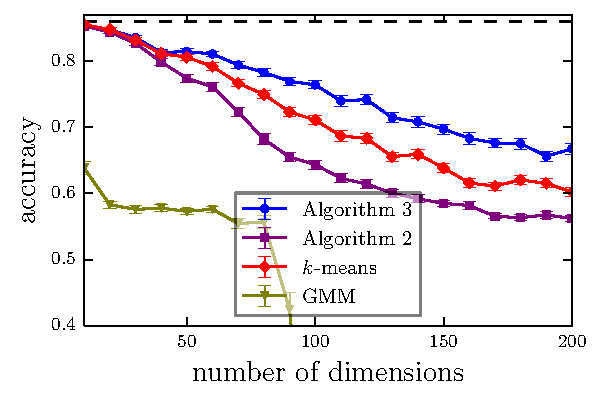
\includegraphics[width=1\textwidth]{gauss_dim.pdf}\\[-1.0em]
(a)
\end{minipage}
\begin{minipage}{0.49\textwidth}
\centering
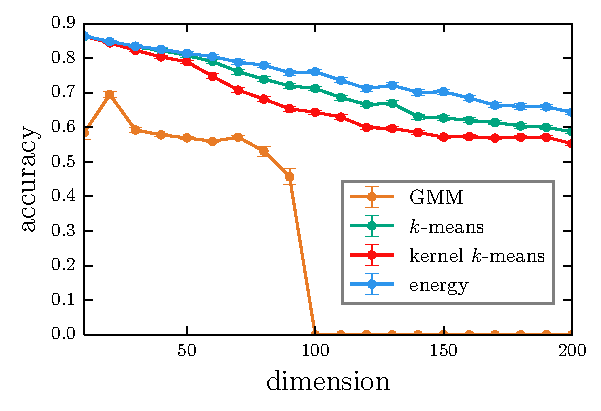
\includegraphics[width=1\textwidth]{gauss_cov.pdf}\\[-1.0em]
(b)
\end{minipage}
\caption{
\label{fig:gauss}
Effect of increasing the
ambient dimension while keeping Bayes error fixed, for 
two clusters with normally distributed data with $100$ points in each
cluster. 
(a) 
We increase $D$ as described in \eqref{eq:gauss1}. The blue
line correspond to Algorithm~\ref{algo}, while
the magenta line 
corresponds to kernel $k$-means, Algorithm~\ref{kmeans_algo}.
(b) The same but with data following \eqref{eq:gauss2}.
One notices that
Algorithm~\ref{algo} is more robust than the other ones.
}
\end{figure}

In Figure~\ref{fig:unbalanced} we consider the effect of having 
unbalanced clusters. We generate data as
\begin{equation}
\label{eq:gauss3}
\begin{split}
&x \sim  
\dfrac{n_1}{N} \mathcal{N}(\mu_1,\Sigma_1) + 
\dfrac{n_2}{N} \mathcal{N}(\mu_2, \Sigma_2), 
\quad \mu_1 = (0,0,0,0)^\top , \,
\mu_2 = 1.5\times (1,1,0,0)^\top, \\
&
\Sigma_1 = I_4, \quad
\Sigma_2 = \left( 
\begin{smallmatrix} 
1/2 & 0 & 0 & 0\\
0 & 1/2 & 0 & 0 \\
0 & 0 & 1 & 0 \\
0 & 0 & 0 & 1 
\end{smallmatrix}\right), \quad
n_1 = N - m, \quad  n_2 = N + m, \quad N=200.
\end{split}
\end{equation}
We then increase $m$, i.e. we make the clusters progressively more unbalanced.
We generate $100$ experiments for each $m$, and plot the clustering accuracy
versus $m$.
As expected, GMM
works better than the other algorithms in the case of unbalanced clusters. 
This is mostly due to its soft assignments.
We can see that the other methods based on hard assignments degrade similarly,
and  more rapidly than GMM. This indicates that a fuzzy version of
energy statistics clustering should compensate for this effect.

\begin{figure}
\centering
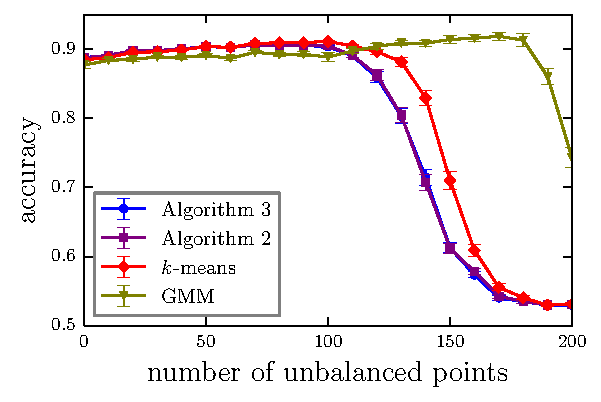
\includegraphics[width=0.5\textwidth]{gauss_pi.pdf}
\caption{
\label{fig:unbalanced}
Previous algorithms for unbalanced clusters, 
according to \eqref{eq:gauss3}.}
\end{figure}

Now, besides \eqref{eq:standard_metric} we consider two other semimetrics:
\begin{align}
\rho_{1/2}(x,y) &= \| x-y \|^{1/2}, & \kk(x,y) &= \tfrac{1}{2} \left( 
\| x \|^{1/2} + \| y \|^{1/2} 
- \| x-y \|^{1/2} \right), \label{eq:rhohalf}\\
\rho_{e}(x,y) &= 2 - 2 e^{-\| x- y\|/2}, & \kk(x,y) &= e^{-\| x-y\|/2}.
\label{eq:rhoe}
\end{align}
In Figure~\ref{fig:consist}a we have data in $20$ dimensions distributed as
\begin{equation}
\label{eq:20gauss}
\begin{split}
x &\sim \tfrac{1}{2}\left[ \mathcal{N}(\mu_1,\Sigma_1) + \mathcal{N}(\mu_2,
\Sigma_2) \right], \\
\mu_1 &= (\underbrace{0,\dotsc,0}_{\times 20})^\top ,\quad
\mu_2 = \tfrac{1}{2} 
(\underbrace{1,\dotsc,1}_{5},\underbrace{0,\dotsc,0}_{15})^\top, \quad
\Sigma_1 = \tfrac{1}{2} I_{20},  \quad
\Sigma_2 = I_{20}.
\end{split}
\end{equation}
We increase the number of points in each cluster and show the clustering
accuracy with different algorithms. The new semimetrics \eqref{eq:rhohalf}
and $\eqref{eq:rhoe}$ are indicated in the legend. One can see that
Algorithm~\ref{algo} performs better than all the other ones, and in 
particular \eqref{eq:rhoe} provides better results.
As the number of datapoints 
get large enough, GMM starts to be as accurate as clustering
based on energy statistics, as it should since it is 
consistent model to the data. In Figure~\ref{fig:consist}b, however, we
use the same parameters as in \eqref{eq:20gauss} but now with data
log-normally distributed:
\begin{equation}
\label{eq:20loggauss}
x \sim \tfrac{1}{2}\left[ e^{\mathcal{N}(\mu_1,\Sigma_1)}
+ e^{\mathcal{N}(\mu_2, \Sigma_2)}\right].
\end{equation}
We see that clustering based on energy statistics still performs accurately
for this kind of data, while $k$-means works a little bit better than chance,
and GMM is not even able to estimate the parameters. Again, \eqref{eq:rhoe}
provides slightly better results than \eqref{eq:standard_metric} or
\eqref{eq:rhohalf}. Notice also that Algorithm~\ref{algo} performs better
than Algorithm~\ref{kmeans_algo}. Both experiments in Figure~\ref{fig:consist}
shows that energy statistics clustering is nonparametric, since it is able
to cluster data coming from very different distributions.

\begin{figure}
\begin{minipage}{0.49\textwidth}
\centering
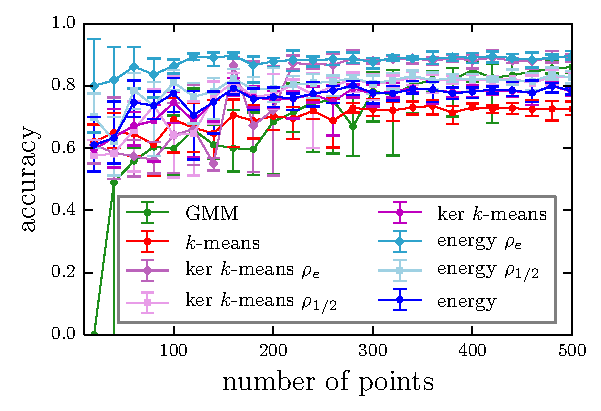
\includegraphics[width=1\textwidth]{gauss.pdf}\\[-1.0em]
(a)
\end{minipage}
\begin{minipage}{0.49\textwidth}
\centering
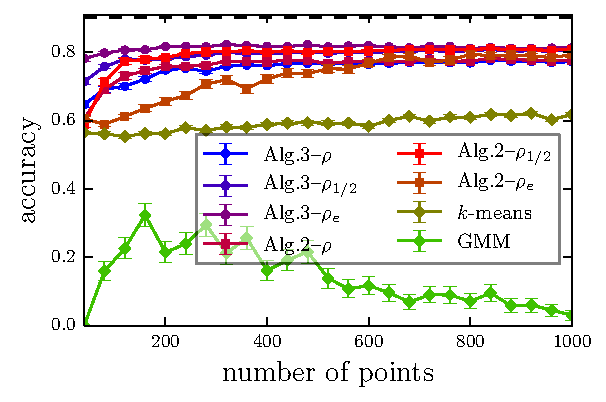
\includegraphics[width=1\textwidth]{loggauss.pdf}\\[-1.0em]
(b)
\end{minipage}
\caption{
\label{fig:consist}
(a) Data normally distributed as in 
\eqref{eq:20gauss}. We increase the number of points in each cluster to
illustrate the statistical consistency of the algorithms.
(b) The same experiment but for data following \eqref{eq:20loggauss}.
In both experiments, for each case we run every algorithm $100$ times and show
the average results. One can see the better performance of energy statistics
clustering, Algorithm~\ref{algo}, and in particular by using the semimetric
\eqref{eq:rhoe}. These two figures illustrate that energy statistics clustering
is nonparametric since it works well for very different distributions.
}
\end{figure}


%%%%%%%%%%%%%%%%%%%%%%%%%%%%%%%%%%%%%%%%%%%%%%%%%%%%%%%%%%%%%%%%%%%%%%%%%%%%%%%
\section{Conclusion}
\label{sec:conclusion}

In this paper we have considered clustering from the perspective of energy
statistics, which provides a nonparametric test for equality of distributions.
Based on this, we showed that the clustering problem reduces to a quadratically
constrained optimization problem (QCQP), 
as described in Proposition~\ref{th:qcqp2}.
Moreover, we showed that clustering based on energy statistics is equivalent
to kernel $k$-means optimization problem, once the kernel is fixed; see
Proposition~\ref{th:kernel_kmeans}. Our results imply that kernel $k$-means
approach to clustering is actually a consequence of energy statistics
theory, and thus place this method into a principled statistical basis.
As already known \cite{Dhillon}, this approach is related to spectral
clustering, and graph partitioning problems. Therefore, all these problems 
may be seen as arising naturally from energy statistics clustering.
It is important to mention that energy statistics clustering, as formulated
here, is valid for
arbitrary metric spaces of negative type, and makes no assumptions about
the distribution of the data. Moreover, it does not rely on the concept of a
cluster mean, even implicitly.

We also proposed Algorithm~\ref{algo} as an alternative to the well-known
kernel $k$-means algorithm (see Algorithm~\ref{kmeans_algo}), 
where both have the same time
complexity. The numerical results show that Algorithm~\ref{algo}
might provide better clustering accuracy and is more robust 
than kernel $k$-means algorithm. Since there exists a huge literature about
kernel $k$-means, and approximation methods to make it faster, with
applications to several artificial and real data, 
we limited ourselves to analyze few but carefully designed experiments, which
illustrates the advantages of Algorithm~\ref{algo}.


\bigskip

%\subsection*{Acknowledgements}
%We thank \ldots


\bibliographystyle{unsrt}
\bibliography{biblio.bib}



\end{document}
